\chapter{\acl{SRS}}
	Das \acf{SRS} ist ein veröffentlichter Standard zur Spezifikation einer Software. Der Inhalt eines \ac{SRS} ist vom Institute of Electrical and Electronics Engineers im Standard IEEE 830-1998 festgehalten.
	
	Der Aufbau dieses Kapitels entspricht der Struktur, die in dem Standard beschriebenen wird. Einige Kapitel des SRS werden allerdings nicht behandelt, da sie keine Relevanz für NoRPG haben oder an einer anderer Stelle in diesem Dokument erwähnt werden.
	
\section{Einführung}
	Das erste Kapitel des \ac{SRS} enthält eine Beschreibung und eine Übersicht über alles, was im \ac{SRS} enthalten ist.
	
	\subsection{Zweck}
		Das \ac{SRS} beschreibt den kompletten Projektumfang und die Anforderungen an die Software NoRPG. Es illustriert den Zweck und die vollständige Erklärung für die Entwicklung der Software. Dabei werden unter anderem Systemeinschränkungen, Schnittstellen und Interaktionen mit externen Schnittstellen thematisiert\footnote{vgl. Tripp \cite{srsIEEE}(1998) Seite 3}. 
	
		Die Zielgruppe des \ac{SRS} bzw. die Stakeholder des Projektes sind alle Personen und Personengruppen, die in irgendeiner Verbindung mit NoRPG stehen oder jene, die Interesse an der Umsetzung haben\footnote{vgl. Rozanski \cite{rozanski2011}(2011) Seite 6}. Zudem dient die Spezifikation zur Kommunikation zwischen den Stakeholdern und den Entwicklern.
		
	\subsection{Umfang}
		Dieses \ac{SRS} handelt von der in Kapitel 2 beschrieben Software NoRPG. 
		
\section{Allgemeine Beschreibung}
	Im zweiten Kapitel des \ac{SRS} werden alle allgemeinen Faktoren, die das Produkt und seine Anforderungen betreffen, beschrieben. Dieses Kapitel bietet einen Überblick über die Systemfunktionalitäten und stellt verschiedene Arten von Stakeholdern und deren Interaktionen mit dem System vor. Dieses Kapitel behandelt jedoch nicht die spezifischen Anforderungen, sondern stellt den Hintergrund für diese dar. 

	\subsection{Produktperspektive}
		Das zu beschreibende vollständige System NoRPG besteht aus mehreren Komponenten, die auf unterschiedlichsten weisen mit den Stakeholdern kommunizieren. Daher ist es besonders wichtig, das Produkt in unterschiedlichen Perspektiven mit verwandten und geplanten Produkten zu betrachten. Aus diesem Grund werden alle System-, Benutzer-, Hardware- und Softwareschnittstellen von NoRPG definiert. 
		
		Folgende Grafik \ref{highlevelview} stellt dabei die High-Level-View von NoRPG und seinen Komponenten dar.

		\begin{figure}[htbp]
			\centering 
			\label{highlevelview}
			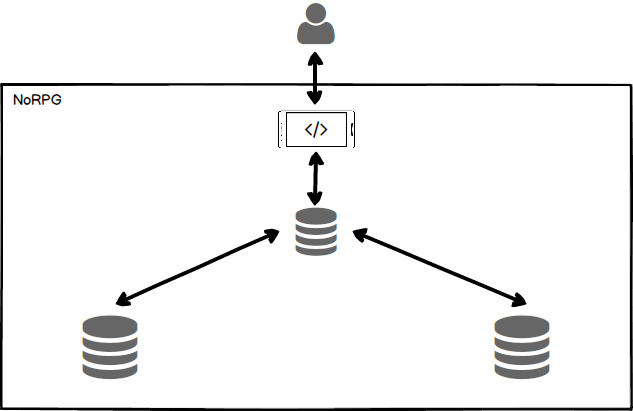
\includegraphics[width=12cm]{pics/HighLevelView.png}
			\caption{High-Level-View von NoRPG}
		\end{figure}
		
		Das vollständige System von NoRPG besteht aus zwei Kernkomponenten. Die erste Kernkomponente ist die Android App, welche sich aus dem Quellcode des Spieles und einer eingebetteten lokalen Datenbank zusammensetzt. Die zweite Kernkomponente ist eine Datenbank, die sich auf einem virtualisierten Server befindet.
		
		Die Schnittstelle zwischen der App und dem Betriebssystem des Smartphones ist eine Systemschnittstelle. Systemschnittstellen identifizieren die Funktionalität der Software, um die Systemanforderung und Schnittstellenbeschreibung zu erfüllen, damit die Software mit dem System übereinstimmt\footnote{vgl. Tripp \cite{srsIEEE}(1998) Seite 13}.
		
		Bei der App NoRPG handelt es sich um die Benutzerschnittstelle des Systems. Benutzerschnittstellen beschreiben die Kommunikation zwischen dem System und dem User. Die Benutzeroberfläche der App ist die einzige Möglichkeit für den Anwender mit dem System zu interagieren.
		
		Jede Schnittstelle zwischen NoRPG und Hardwarekomponenten des Systems werden als Hardwareschnittstellen bezeichnet. Das Smartphone mit all seinen Komponenten sind Hardwarekomponente, zu der eine direkte  Schnittstelle existiert. Die Hardwarekomponenten eines Smartphones sind der Touchscreen, die Lautsprecher oder der WLAN-Adapter. Diese Komponenten werden in der Abbildung durch das Smartphone zusammengefasst. Eine weitere Hardwareschnittstelle gibt es zwischen dem Server und der Hardware, auf dem dieser installiert ist.
		
		Die App kommuniziert mit der lokalen, sowie mit der serverseitigen Datenbank und verwendet dabei die Funktionen von anderen Softwareprodukten. Dabei handelt es sich um Softwareschnittstellen. Sie bilden den Übergang zwischen unterschiedlichen Programmen und ermöglichen dadurch das Nutzen derer Funktionalitäten. 

	\subsection{Produktfunktionen}
		In diesem Unterkapitel werden die wichtigsten Funktionen von NoRPG zusammengefasst. Wie in Kapitel 2 beschrieben ist das Hauptziel von NoRPG Lernspiele in einer standardisierten Reihenfolge zum Herunterladen anzubieten. Dieses Ziel macht das Downloaden von Spielen zu der Hauptfunktionalität von NoRPG. 
		
		Neben dieser Funktion gibt es allerdings weitere Produktfunktionen, um NoRPG attraktiver zu gestalten und zu personalisieren. Der Spieler wird in der Lage sein mit Elementen im Spiel zu interagieren und dabei Spielgegenstände zu sammeln. Um dem Anwender eindeutig identifizieren zu können, wird NoRPG über eine eigene Anmelde- und Registrierungsfunktion verfügen. In diesem Registrierungsprozess ist es dem Spieler möglich, seinen eigenen persönlichen Charakter zu erstellen.
		
		Im Spiel selbst wird es neben Spieloptionen wie Qualitäts- und Audioeinstellungen noch Features geben, die das Spielerlebnis verbessern sollen. Dazu zählen Funktionen wie das öffnen einer Karte der aktuellen Spielwelt oder das betrachten des Fortschritts im jeweiligen Standard.
		
		Die App speichert den Fortschritt und die Daten in der lokalen eingebetteten Datenbank und synchronisiert diese Informationen mit dem Server.
	
	\subsection{Benutzermerkmale}
		Im Rahmen dieser Studienarbeit wird zunächst nur eine Benutzergruppe vollständig implementiert und daher nur diese hier beschrieben.
		
		Die zu implementierende Benutzergruppe sind die User, viel mehr die Spieler. Grundsätzlich richtet sich NoRPG an Kinder, die keine Möglichkeit haben eine Schule zu besuchen. Jedoch werden keine Benutzergruppen für diese App ausgeschlossen. Egal ob jung oder alt, männlich oder weiblich, der Spieler sollte nur eine Neugier zum Lernen mitbringen. 
		
		Der Anwender benötigt Erfahrung mit der Verwendung eines Smartphones, insbesondere mit einem Android-Systems. Dazu zählt die Bedienung der Android-Oberfläche und die des Google Play Stores. Zudem sollten die User englische Texte lesen und verstehen können, da NoRPG zunächst nur in Englisch erscheinen wird.
			
	\subsection{Einschränkungen}
		Da das \ac{SRS} für die Kommunikation zwischen Entwickler und Stakeholder dient, wird zwischen Einschränkungen für Entwickler und für Spieler unterschieden.
		
		Grundsätzlich müssen sich Entwickler an die vorgegebenen regulatorischen Richtlinien, wie beispielsweise an die Datenschutzerklärung von Google oder an das IT-Sicherheitsgesetz halten.
		
		Da NoRPG sich an Kinder in bildungsfernen Ländern richtet ist es besonders wichtig, dass die Texte in NoRPG einfach zu verstehen sind. Da das Spiel zunächst nur in Englisch erscheinen wird, dürfen die englischen Texte kein Fachjargon oder ähnliches beinhalten. Die App darf keine hohen Mindestanforderungen an Hardwareressourcen haben, da der technische Standard in bildungsfernen Ländern geringer ist. Das bedeutet für die Entwickler das Spiel so gut wie möglich ressourcenschonend umzusetzen. Des Weiteren gilt es bei der Implementierung zu beachten, dass NoRPG soweit wie möglich ohne eine aktive Internetverbindung spielbar bleiben muss.
		
		Allerdings gibt es auch Einschränkungen, welche für die Spieler gelten oder zumindest temporär. Wie schon öfter erwähnt wurde, wird das Spiel zunächst nur in Englisch erscheinen. Dementsprechend benötigt der Spieler Englischkenntnisse um die Texte im Spiel lesen und verstehen zu können. Für die Anmeldung, die Registrierung, das Herunterladen von Spielen, das Synchronisieren und installieren von Updates wird eine aktive Internetverbindung vorausgesetzt. Des Weiteren benötigt der Spieler ein Android Smartphone, welches die Mindestanforderungen von NoRPG erfüllt.
				
	\subsection{Annahmen und Abhängigkeiten}
		Eine Annahme von NoRPG ist, dass es immer auf Smartphones, die genügend Leistung haben, verwendet wird. Wenn das Telefon nicht über genügend Hardwareressourcen für die Anwendung verfügt, kann es Szenarien geben, in denen die Anwendung nicht wie beabsichtigt oder überhaupt nicht funktioniert.
		
		Eine weitere Annahme ist, dass das Smartphone und dessen Hardware sowie Software funktionieren. Das Smartphone muss sich mit dem Internet verbinden können, wenn der Benutzer sich anmelden möchte oder Lernspiele herunterladen will. Neben einer funktionierenden Internetverbindung sollten andere Hardwareelemente wie die Lautsprecher oder der Touchscreen funktionieren. Das Smartphone muss eine gültige Android Version mit einem Google Konto besitzen.
		
	\subsection{Aufteilung der Anforderungen}
		In dem Fall, dass das Projekt verzögert wird, gibt es einige Anforderungen, die auf die nächste Version der Anwendung übertragen werden könnten.

\section{Spezifische Anforderungen}
	Das letzte Kapitel des \ac{SRS} dient dazu alle Anforderungen an die Software detailliert zu beschreiben. Dies ermöglicht es Entwicklern ein System zu entwickeln, welches allen Anforderungen entspricht, und Testern, NoRPG ausreichend zu testen.
	
	\subsection{Externe Schnittstellen}
		Dieser Abschnitt ist die detaillierte Beschreibung aller Ein- und Ausgänge von NoRPG. Diese Beschreibung ergänzt und vervollständigt die Schnittstellenbeschreibung von Kapitel 2.2.1. 
	
		\subsubsection{Systemschnittstellen}
			NoRPG hat genau eine Schnittstelle mit einem anderen System und zwar mit Android. Android ist das Betriebssystem von Google für mobile Geräte, welches aktuell in der Version 7.1 Nougat zu erhalten ist. Viele Smartphone-Hersteller nutzen Android als Basis für ihr eigenes auf Android aufbauendes Betriebssystem. 
			
			Der Gültigkeitsbereich der Systemschnittstelle ist auf die App begrenzt und hat keinerlei direkte Auswirkungen auf den Server. 
			
			Das Datenformat von Android ist das \ac{APK} und wird für die Distribution und Installation von mobilen Apps auf Android Smartphones verwendet. Eine \ac{APK}-Datei enthält den gesamten Programmcode, Ressourcen, Assets, Zertifikate und Metadaten. Verglichen kann das Datenformat von Google mit einem ZIP-Archiv\footnote{vgl. Dan Morrill (Google) \cite{google1}}. Dieses Format muss NoRPG erfüllen, um unabhängig von den zu implementierenden Produktfunktionen auf einem Android Smartphone laufen zu können.
			
		\subsubsection{Benutzerschnittstellen}
			Die Benutzerschnittstellen bzw. \ac{UI} sind der Punkt, an dem die Benutzer mit der Software interagieren. Zur Beschreibung der Benutzerschnittstellen werden logische Eigenschaften und Aspekte zur Optimierung formuliert. Für die Veranschaulichung werden Mockups verwendet. Diese stellen dar, wie die Oberfläche aussehen kann. Die am Projektende implementierte Benutzeroberfläche kann sich von den Mockups unterscheiden.
			
			Wenn der Benutzer NoRPG das erste Mal startet oder nicht angemeldet ist, wird ihm die Login-Oberfläche (siehe Abbildung \ref{mockupLogin}) präsentiert. Auf dieser Oberfläche hat der Benutzer die Möglichkeit sich mit seinem Benutzernamen und Passwort anzumelden oder sich, falls noch nicht geschehen, bei NoRPG zu registrieren. Das Smartphone muss Quer gehalten werden, da alle Elemente des Bildschirms für diese Ausrichtung angeordnet sind. Diese Eigenschaft gilt ebenfalls für alle anderen Benutzerschnittstellen und wird nicht bei den Beschreibungen der anderen \acp{UI} zusätzlich erwähnt.  
			
			Die Hauptelemente des Login-Screens sind die Eingabefelder für Benutzername und Passwort, der Login- und Registrierungsbutton sowie ein Ladebalken, der den aktuellen Status von NoRPG zeigt. Wenn das Spiel aktualisiert wird kann hier der Status abgelesen werden. Zur Optimierung der Nutzung ist das Layout der Login-Oberfläche ein Border-Pane, in dem die Bestandteile in einer einzigen Spalte angeordnet sind. Fehler werden in einem kleinen Fenster dargestellt, wenn beispielsweise der Benutzer falsche Login-Daten eingibt oder die Internetverbindung während des Aktualisierungsprozesses abbricht.

			\begin{figure}[htbp]
				\centering 
				\label{mockupLogin}
				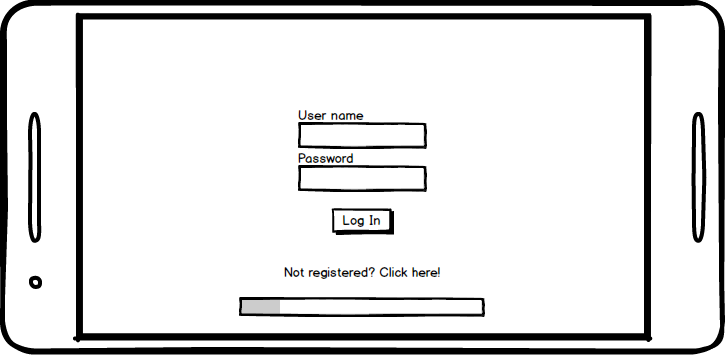
\includegraphics[width=10cm]{pics/Login.png}
				\caption{Mockup: Login-Screen}
			\end{figure}
			
			Falls sich der Benutzer bei NoRPG registrieren möchte, hat er die Möglichkeit dies den Namen, das Geschlecht und Aussehen seines Charakters.
			irekt in der App zu machen. Dazu klickt der Benutzer den Register-Button auf der Login-Oberfläche. Anschließend öffnet sich die Register-Oberfläche. Der vollständige Registrierungsprozess (siehe Abbildung \ref{mockupsRegistrierung}) setzt sich aus zwei Schritten zusammen. Im ersten Schritt muss der Spieler das Registrierungsformular ausfüllen und bestätigen. Die Elemente des Formulars sind als Tabellen-Layout angeordnet, welches die Lesbarkeit verbessert. Felder, die nicht der erwarteten Eingabe entsprechen, werden als Falsch markiert und visuell hervorgehoben. Wenn das Anlegen des Accounts erfolgreich war, hat der Anwender die Möglichkeit im zweiten Schritt seinen persönlichen Charakter zu erstellen. Dafür bestimmt der Benutzer d
			\begin{figure}[htbp]
				\centering 
				\label{mockupsRegistrierung}
				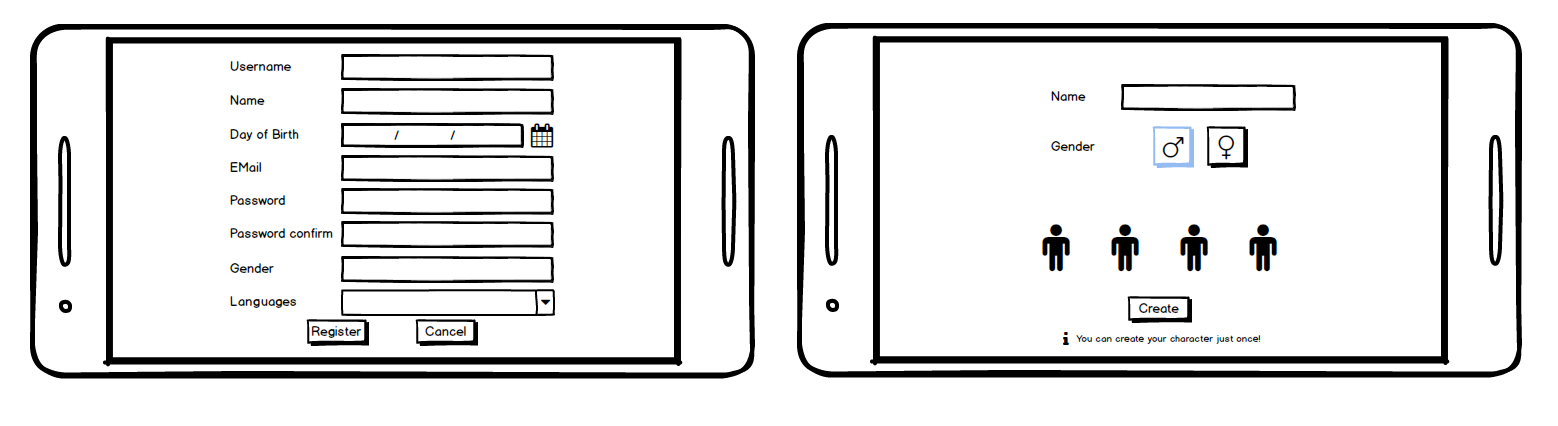
\includegraphics[width=\textwidth]{pics/Registerprozess.png}
				\caption{Mockups: Registrierungsformular und Charaktererstellung}
			\end{figure}
		
			NoRPG startet erst, nachdem alles geladen wurde und der Benutzer angemeldet ist. Der Bildschirm von NoRPG besteht aus der Spielwelt (Grafik) und dem \ac{HUD}. Das \ac{HUD} ist eine Methode, mit der Informationen visuell als Teil der Benutzeroberfläche eines Spiels vermittelt werden. Während die Informationen, die auf dem \ac{HUD} angezeigt werden, stark vom Spiel abhängen, gibt es viele Eigenschaften, die Spieler über viele Spiele erkennen. Die meisten von ihnen sind statisch auf dem Bildschirm, so dass sie während des Spiels sichtbar bleiben.  
			
			\begin{figure}[htbp]
				\centering 
				\label{mockupHUD}
				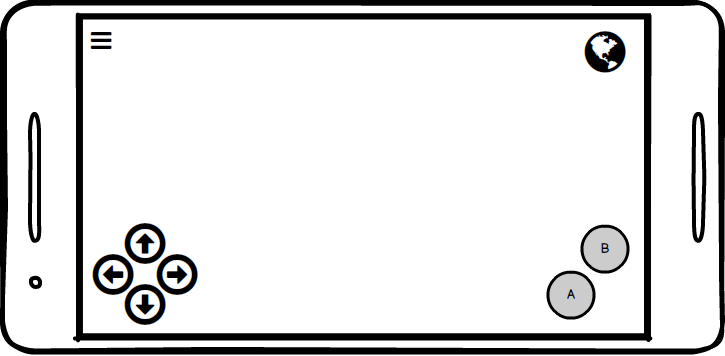
\includegraphics[width=10cm]{pics/HUD.png}
				\caption{Mockup: Head-Up Display}
			\end{figure}
			
			Das Mockup in Abbildung \ref{mockupHUD} enthält alle direkt sichtbaren \ac{HUD} Elemente, die während des Spieles aktiv sind. Diese Elemente sind an die Ecken des Bildschirmes gebunden, so befinden sich beispielsweise die Pfeiltasten zur Bewegung des Charakters in der linken unteren Ecke des Bildschirms und die Buttons zur Interaktion mit dem Spiel in der unteren rechten Ecke. 
			
			Das Menü (siehe Abbildung \ref{mockupMenu}), welches sich in der oberen linken Ecke befindet, kann geöffnet werden. Dadurch verändert sich das \ac{HUD} von NoRPG und es erscheinen neue Elemente, die der Spieler sehen und benutzen kann. NoRPG ist derweil pausiert. Die anderen Elemente hingegen werden überdeckt oder reagieren nicht solange das Menü offen ist. Deshalb ergeben sich neue Optionen bzw. Möglichkeiten für den Spieler um mit NoRPG zu interagieren.
			
			\begin{figure}[htbp]
				\centering 
				\label{mockupMenu}
				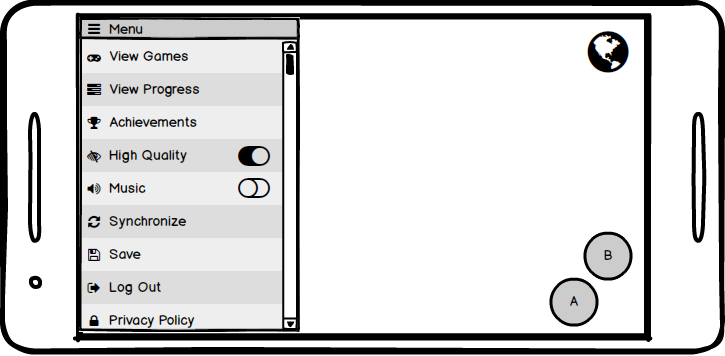
\includegraphics[width=10cm]{pics/Menu.png}
				\caption{Mockup: Menü}
			\end{figure}
			
			Es wird zwischen zwei Typen von Menü-Funktionen unterschieden. Eine Funktionen können direkt im Menü durchgeführt werden, wie beispielsweise die Qualitätseinstellung. Einige der Funktionen wiederum öffnen ein Fenster bzw. eine neue Ansicht, in dem die neuen Funktionalitäten zur Verfügung stehen. Die Fenster müssen erst geschlossen werden, um das Spiel fortsetzen zu können. Beispiele sind in der folgenden Abbildung \ref{mockupFenster} als Mockups zu betrachten.
			
			\begin{figure}[htbp]
				\centering 
				\label{mockupFenster}
				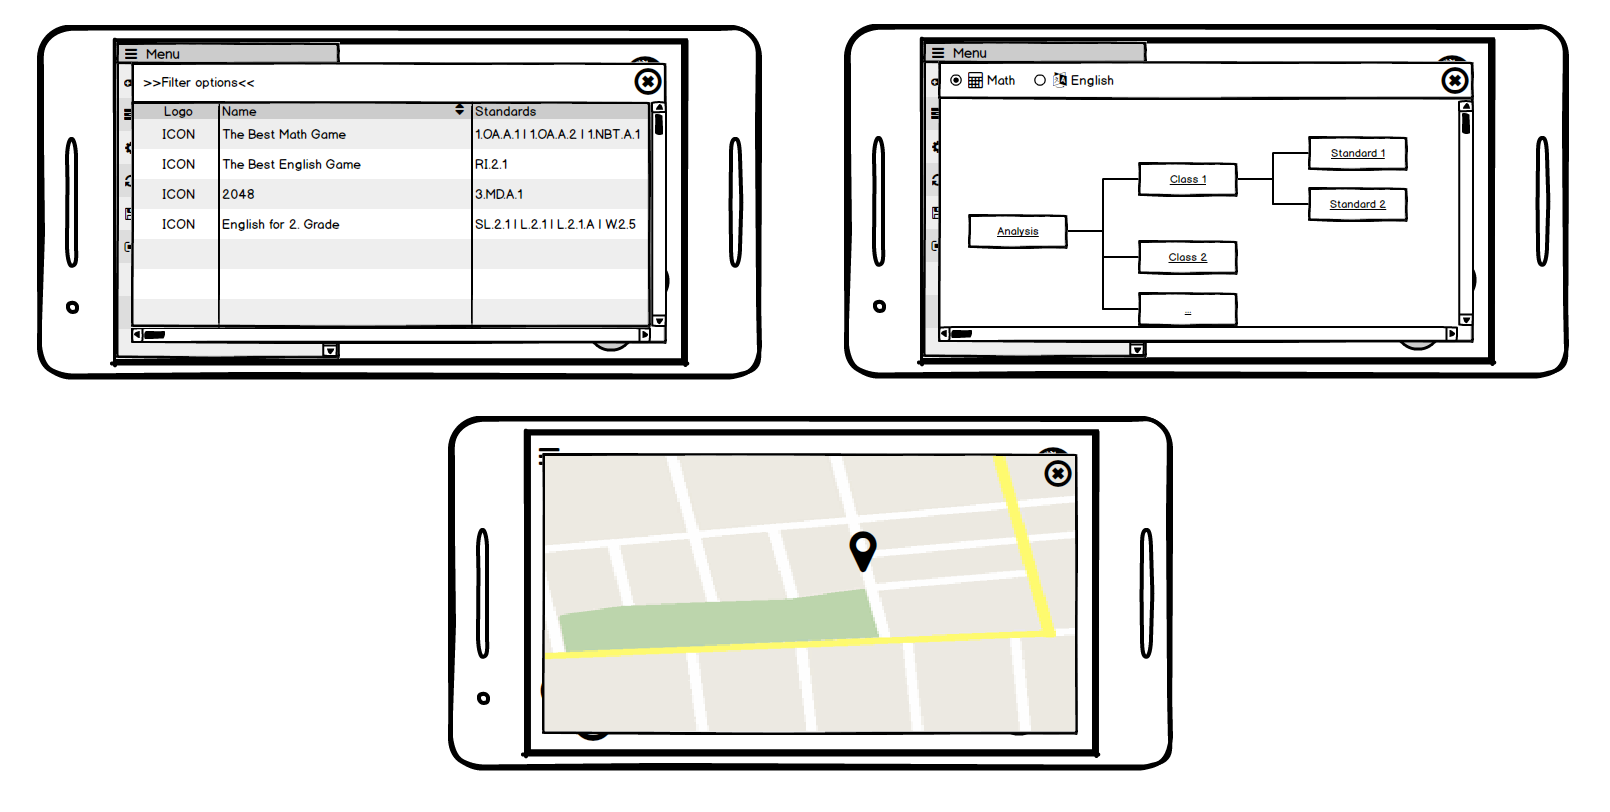
\includegraphics[width=\textwidth]{pics/NewWindows.png}
				\caption{Mockups: Spielliste, Fortschrittanzeige, Karte und Erfolgsübersicht}
			\end{figure}
		
		\subsubsection{Hardwareschnittstellen}
			Schnittstellen zwischen NoRPG und Hardwarekomponenten werden als Hardwareschnittstellen des Systems bezeichnet. Dieses Kapitel dient zur Spezifikation der logischen Eigenschaften dieser Schnittstellen.
			
			Ein Smartphone besteht aus sehr vielen Hardwarekomponenten. Jede einzelne Komponente wird benötigt, damit das Smartphone mit seinem kompletten Funktionsumfang lauffähig ist. Jedoch spielen einige Hardwarekomponenten eine besondere Rolle für NoRPG. Neben unverzichtbaren Komponenten wie den Prozessor, Speicher oder Akku zählen zu den Kernkomponenten der Touchscreen und der WLAN-Adapter. Der Touchscreen wird benötigt um die Eingaben des Spielers an das Spiel zu kommunizieren. Se es die Steuerung des Charakters, das Ausfüllen des Registrierungsformulars oder das einfache betätigen eines Buttons. Ohne den Touchscreen können keine Eingaben ohne zusätzliche Peripherie an das Spiel kommuniziert werden. Der WLAN-Adapter ist zuständig für die Verbindung mit dem Internet. Ohne eine Internetverbindung ist nicht einmal der Login funktionsfähig bzw. es wäre nicht ohne Umstände möglich NoRPG aus dem Google Play Store herunterzuladen.
			
			Obwohl es sich bei dem Server um einen virtuellen bzw. simulierten Server handelt, weiß NoRPG nicht, dass keine physische Hardware direkt benutzt wird. Für die App scheint es, als ob sie mit einem physischen Server kommuniziert. Auch hier sind alle Komponenten des Server, auch wenn diese Simuliert sind, Teil der Hardwareschnittstelle.
			
		\subsubsection{Softwareschnittstellen}
			Softwareschnittstellen spezifizieren die Schnittstellen mit anderen benötigten Softwareprodukten, welche die Nutzung derer Funktionalitäten ermöglicht.
			
			Die vorinstallierte Software Google Play Store ist eine Plattform, die Musik, E-Books, Filme, Serien und insbesondere Apps anbietet. Der Google Play Store stellt eine Softwareschnittstelle zu NoRPG dar. NoRPG benötigt die Schnittstelle zur Spielplattform von Android, um die dort verfügbaren Lernspiel in NoRPG anzuzeigen bzw. als Download anzubieten.
			
			Für die Verarbeitung der Toucheingaben gibt es ein C\# Skript. Erst mit Hilfe dieser Software wird es möglich die Toucheingaben an das Spiel zu kommunizieren, damit die richtige Aktion in NoRPG ausgeführt wird.
			
			Damit die lokalen Datenbanken der Clients und die Datenbank auf dem Server immer synchronisiert bleiben wird eine Datenbanksynchronisationssoftware benötigt, welcher die Synchronisation bei aktiver Internetverbindung übernimmt. Dabei handelt es sich um eine Softwareschnittstelle, da NoRPG die Funktionalität dieser Software verwendet.
			
			Die letzte Softwareschnittstelle ist das \ac{DBMS}. Das \ac{DBMS} ist die Verwaltungssoftware der Datenbank. Sie organisiert intern die strukturierte Speicherung der Daten und kontrolliert alle lesenden und schreibenden Zugriffe auf die Datenbank. Sie wird benötigt um den aktuellen Stand des Spieles zu speichern.

	\subsection{Funktionale Anforderungen}
		Use Cases dokumentieren Funktionalitäten eines Systems auf Basis von einfachen Modellen. In einem Use Case wird das nach außen sichtbare Verhalten eines Systems aus der Sicht des Nutzers beschrieben. Ein Nutzer kann hierbei eine Person, eine Rolle oder ein anderes System sein. Dieser Nutzer tritt als Akteur mit dem System in Interaktion, um ein bestimmtes Ziel zu erreichen.
		
		Use Cases verwenden Activity Diagramme. Ein Activity Diagramm ist ein Verhaltensdiagramm der Unified Modeling Language (UML) und stellt die Vernetzung von elementaren Aktionen und deren Verbindungen mit Kontroll- und Datenflüssen grafisch dar.
	
		\begin{figure}[htbp]
			\centering 
			\label{oucd}
			
\includegraphics[width=11cm]{pics/OUCD.pdf}
			\caption{Overall Use Case Diagramm}
		\end{figure}
		
		Das abgebildete System in Abbildung \ref{oucd} stellt die zu entwickelnde App für die User dar. Die App von NoRPG stellt die graphische Oberfläche und somit die beschrieben Benutzerschnittstellen dar. Es sind nur die Funktionalitäten enthalten, die der Benutzer ausführen kann, also jene die über die Benutzerschnittstellen angesprochen werden können. 
		
		Use Cases wie Login oder Registrierung sind im Overall Use Case Diagramm nicht enthalten, da diese im Vergleich zu anderen Use Cases primitiv sind. Die abgebildeten Use Cases enthalten meistens mehrere Schritte bis die Aktion ausgeführt wird.
	
		\subsubsection{Create character}
			Dieser Use Case beschreibt den Anwendungsfall, dass der Benutzer seinen Charakter erstellen möchte. Dieser Use Case wird pro Account genau einmal im Registrierungsprozess ausgeführt.
			
			Nach erfolgreicher Registrierung kann der Spieler seinen Charakter erstellen. Der User kann den Namen, das Geschlecht und das Aussehen des Charakters bestimmen. Ein möglicher Ablauf des Erstellungsprozesses kann aus Abbildung \ref{createCharakter} entnommen werden.
			
			\begin{figure}[htbp]
				\centering 
				\label{createCharakter}
				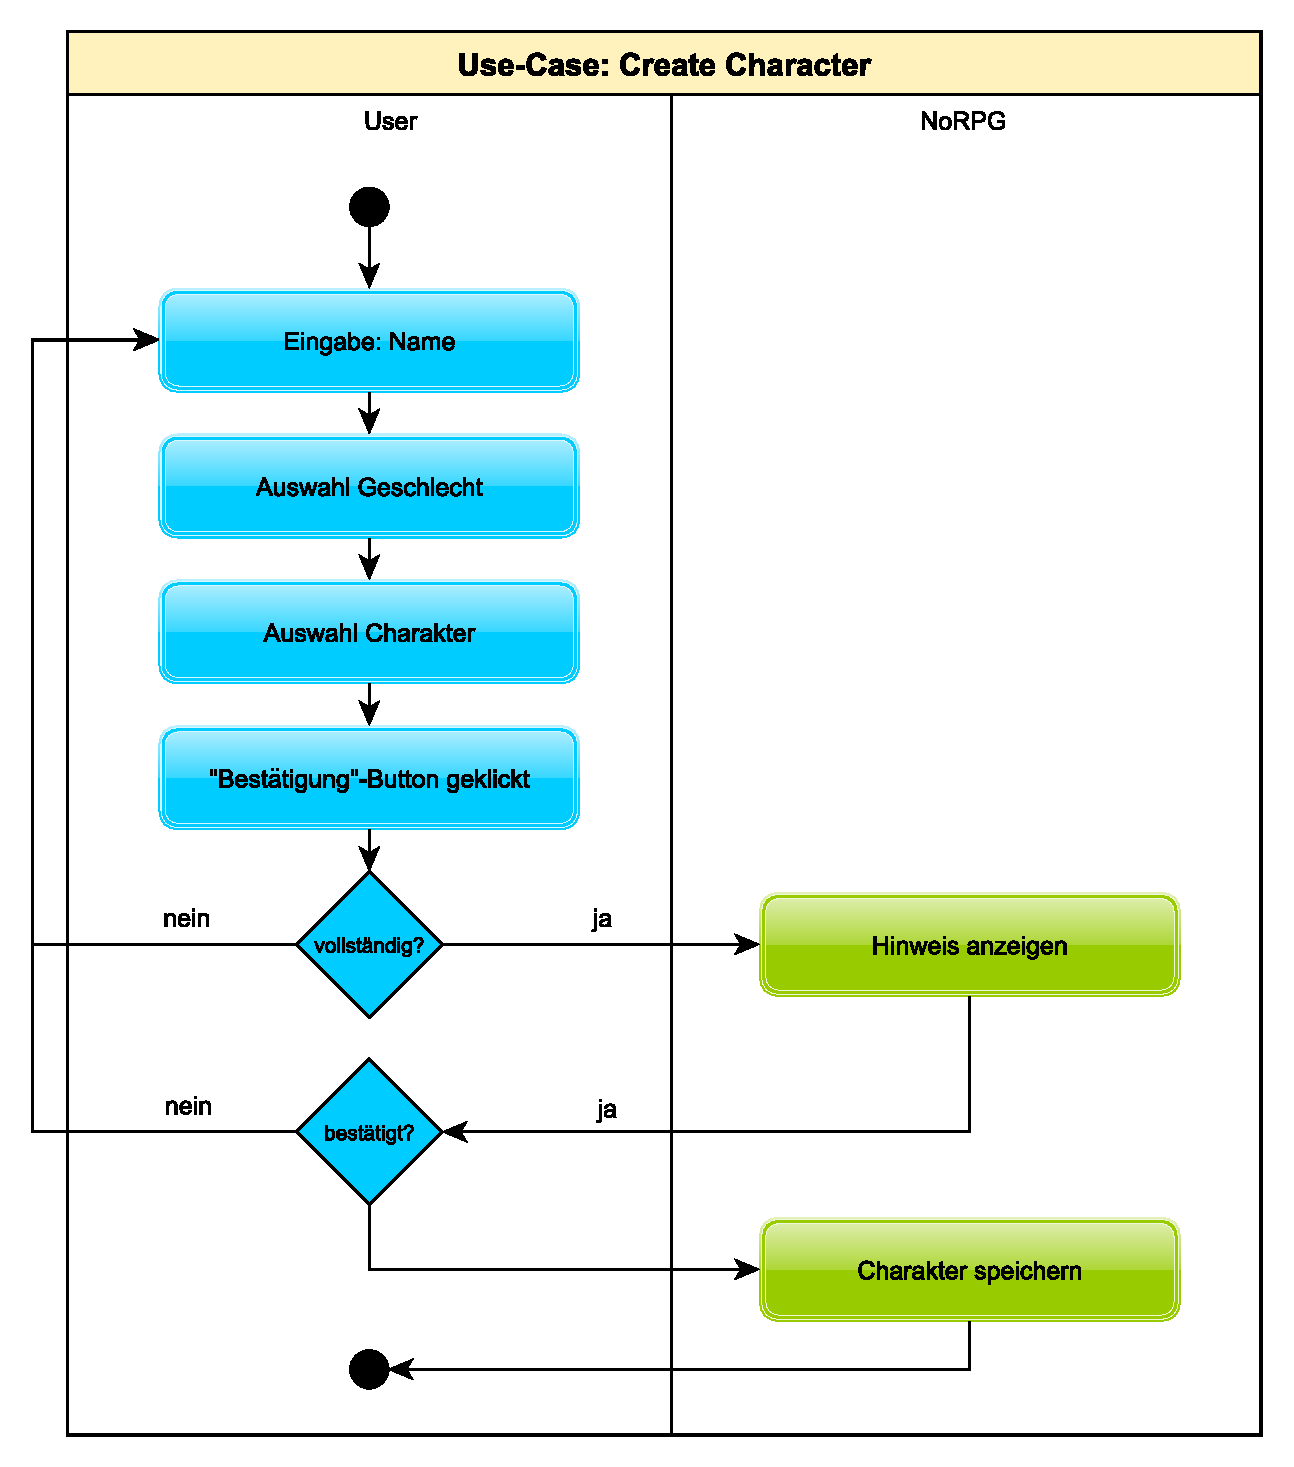
\includegraphics[width=10cm]{pics/CreateCharacter.pdf}
				\caption{Activity Diagramm: Create Character}
			\end{figure}
		
			Der Ablauf des Prozesses kann allerdings variieren. Der Spieler kann beispielsweise erst das Geschlecht und das Aussehen bestimmen und anschließend seinem Charakter einen Namen geben. Die Variationen können allerdings nur bei den Charaktereigenschaften auftauchen.
	
			Bevor jedoch dieser Use Case ausgeführt werden kann, muss der Spieler das Registrierungsformular vollständig ausfüllen und erfolgreich abschließen. Zudem darf Account noch nicht existiert. Für den gesamten Registrierungsprozess ist eine aktive Internetverbindung notwendig, damit der neu angelegte Account mit den Spielereigenschaften direkt mit dem Server synchronisiert werden kann.
			
			Nach der erfolgreichen Erstellung des Charakters, wird dieser in die Datenbank gespeichert und der User kann sich nun anmelden und Spiel starten. Sollte die Erstellung allerdings fehlschlagen, wird der User wieder auf den Hauptbildschirm von NoRPG weitergeleitet. 
			
		\subsubsection{Open map}
			Dieser Use Case beschreibt den Anwendungsfall, dass der Benutzer die Karte der Spielwelt öffnet. Die Karte dient zur Orientierung und kennzeichnet den Aufenthalt des Spielers.
			
			Der Anwender kann die Karte der aktuellen Spielwelt durch einen Klick auf die Mini-Map öffnen. Das Acitivity Diagramm in Abbildung \ref{umlOpenMap}) zeigt den vollständigen Ablauf.
			
			\begin{figure}[htbp]
				\centering 
				\label{umlOpenMap}
				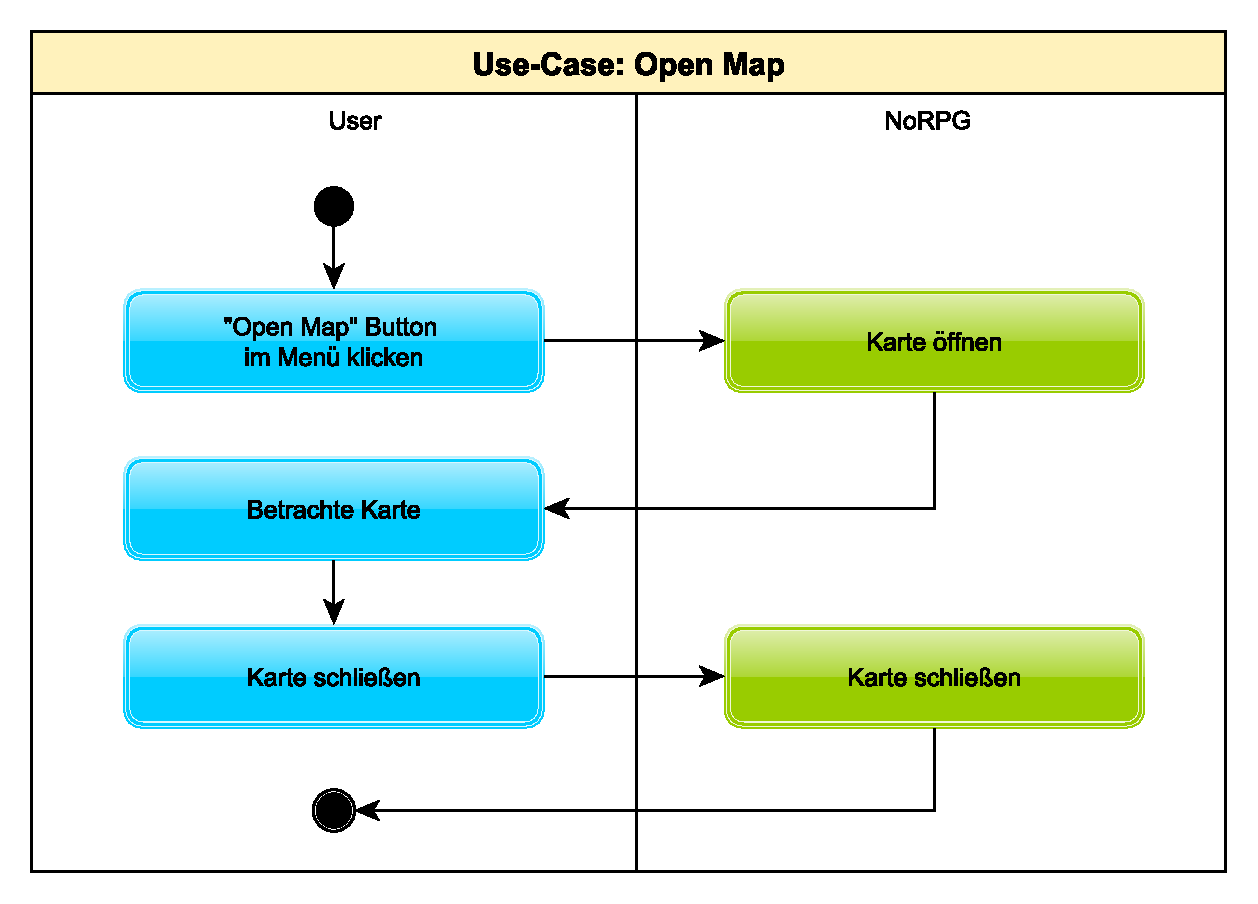
\includegraphics[width=10cm]{pics/OpenMap.pdf}
				\caption{Activity Diagramm: Open Map}
			\end{figure}
			
			Die Vorbedingungen für diesen Use Case sind, dass der Spieler sich im Spiel befindet, das Menü geschlossen ist und der Spieler sich in keiner aktiven \ac{NPC} Interaktion befindet.
			
			In einem Fehlerfall sollte sich die Karte schließen und der Benutzer wieder zum Spiel weitergeleitet werden.
	
		\subsubsection{View games}
			Dieser Use Case beschreibt den Anwendungsfall, dass der Benutzer die Liste der freigeschalteten und spielbaren Spiele öffnen will. Gefundene Spiele in NoRPG werden in diese Liste aufgenommen, so dass der Spieler an einem zentralen Ort alle spielbaren Lernspiele anschauen kann. Die Liste enthält den Namen des Spiels, einen Download-Link sowie die Zuordnung zum entsprechenden Standard. Dadurch ist es möglich auch ohne eine aktive Internetverbindung in NoRPG voranschreiten zu könne.
			
			Das Activity Diagramm in Abbildung \ref{umlShowGames} hat im Vergleich zu den bisherigen betrachteten Activity Diagrammen eine Besonderheit. Die Aktivität "Google Play Store öffnen" findet außerhalb von NoRPG statt. Nach Beendigung diesen Schrittes wird der Spieler wieder zurück ins Spiel weitergeleitet. Allerdings wenn der Prozess von NoRPG währenddessen abgebrochen wird, startet das Spiel am letzten Speicherpunkt. Der Prozess beginnt indem der Spieler die Funktion im Menü aufruft.
			
			\begin{figure}[htbp]
				\centering 
				\label{umlShowGames}
				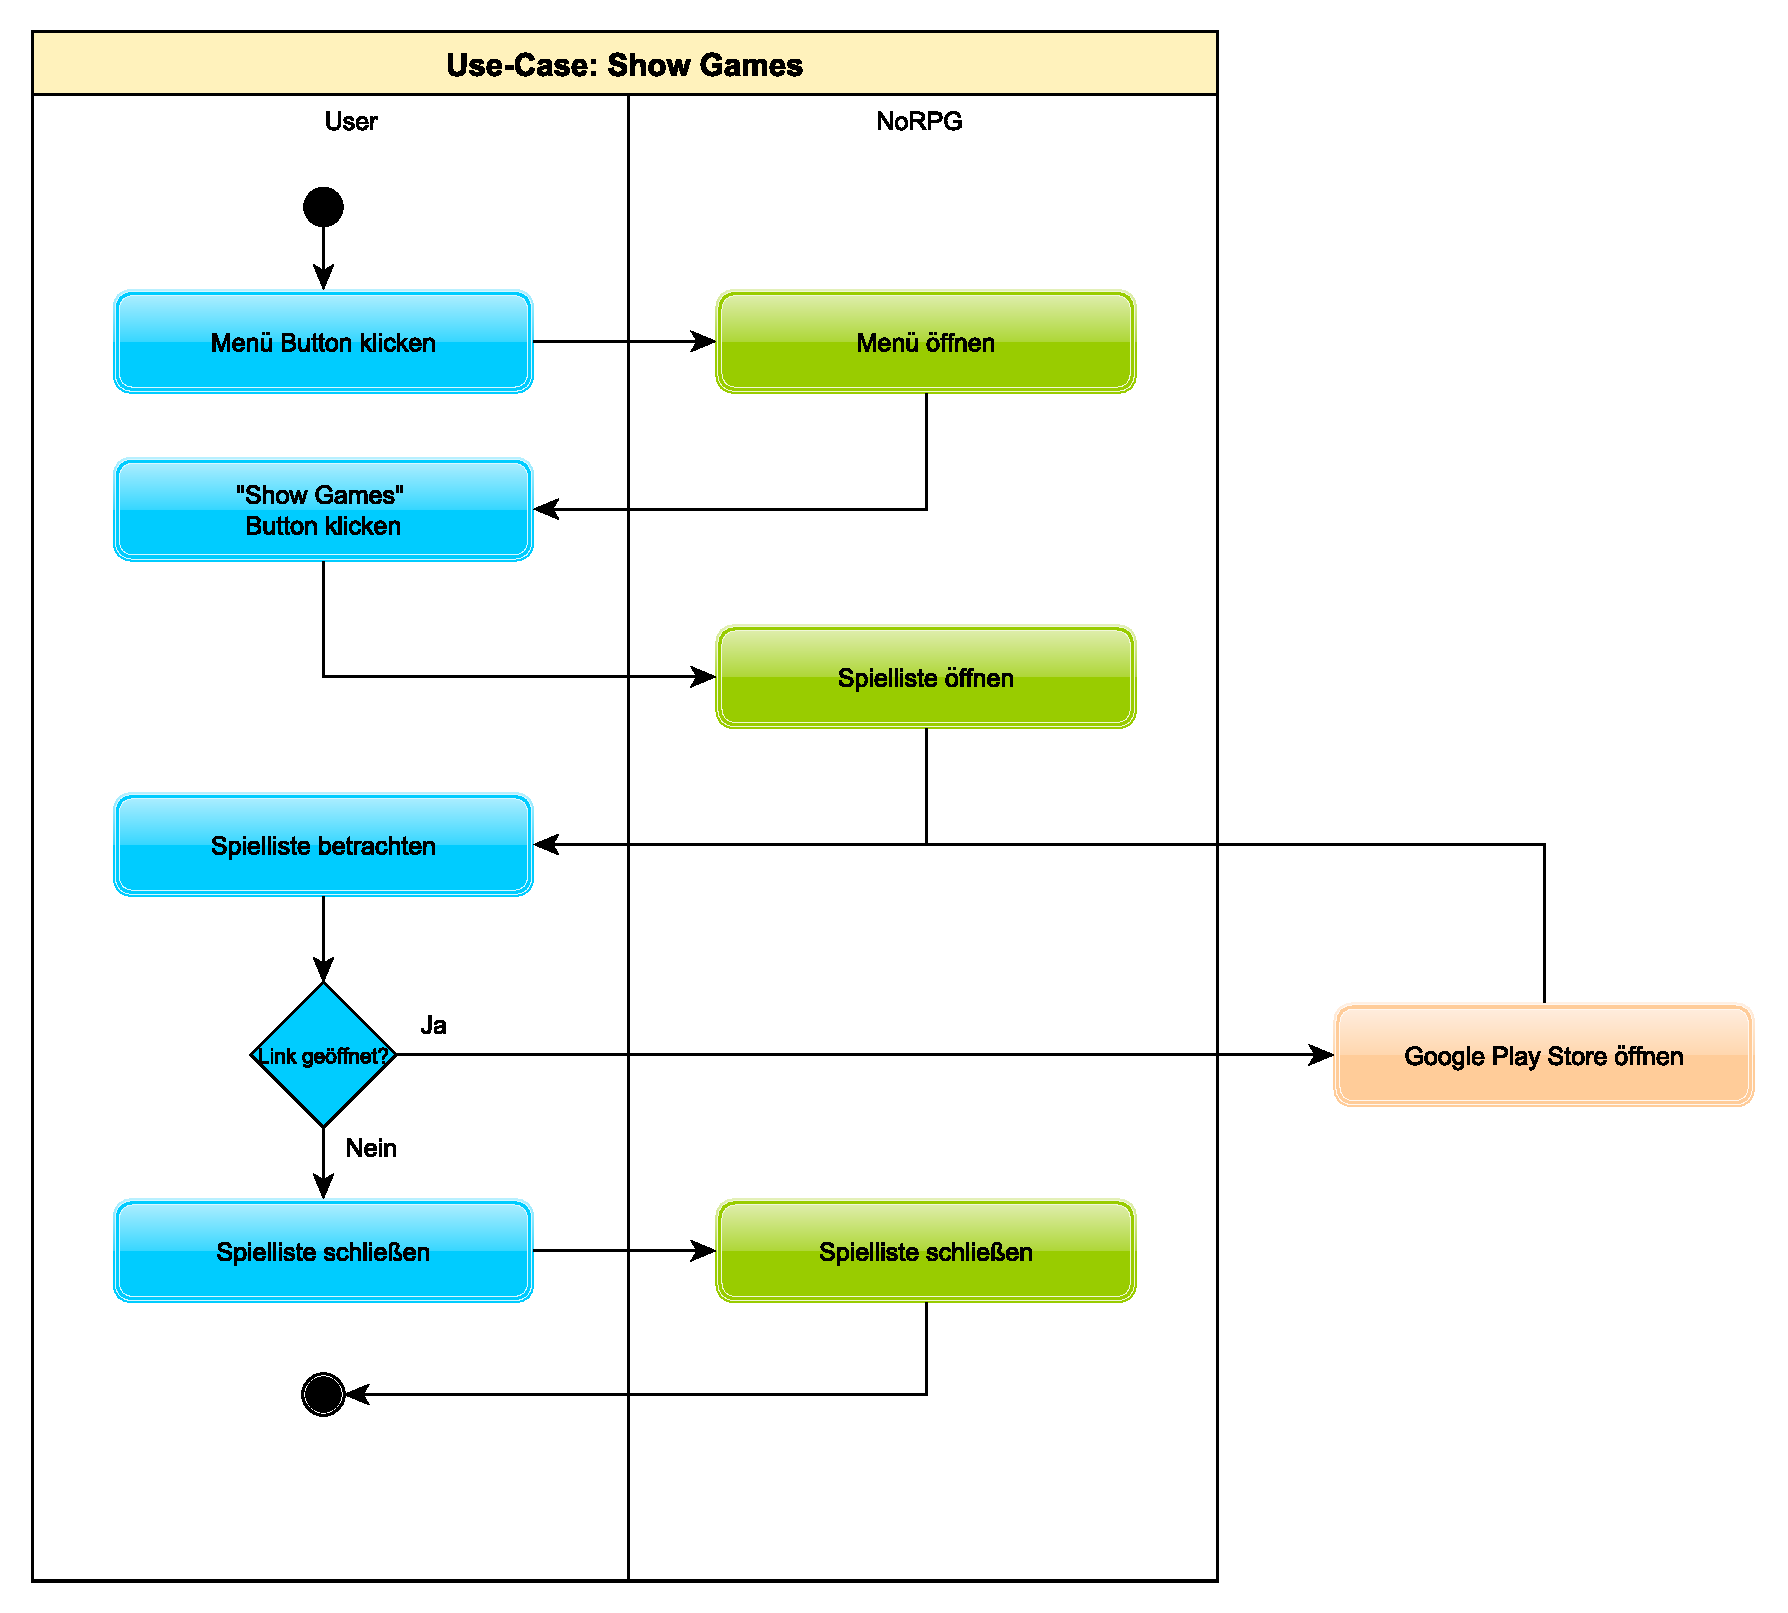
\includegraphics[width=12cm]{pics/ShowGames.pdf}
				\caption{Activity Diagramm: Show Games}
			\end{figure}

			Der Benutzer muss sich im Spiel befinden und darf in keiner aktiven \ac{NPC} Interaktion sein. Zudem muss das Menü vorher offen sein bevor dieser Use Case ausgeführt werden kann. Auch hier gilt im Fehlerfall, dass der Spieler wieder zurück ins Spiel kommt.
	
		\subsubsection{View progress}
			Dieser Use Case beschreibt den Anwendungsfall, dass der Benutzer seinen Fortschritt in NoRPG betrachten möchte. Dafür wird dem Spieler pro Schulfach jeweils ein Baumdiagramm präsentiert, der die Standards und deren Reihenfolge beinhaltet. Durch eine Kennzeichnung kann der Spieler sehen welche Standards abgeschlossen sind und fehlen.  
			
			Das Activity Diagramm in Abbildung \ref{umlViewProgess} ähnelt dem vom Use Case "View Games". Die einzige Ausnahme dabei ist, dass dieses Diagramm keine Aktion hat, die außerhalb von NoRPG stattfindet. Die Fortschrittsanzeige wird im Menü geöffnet. Nachdem die Anzeige offen ist kann der Spieler zwischen den Standards wechseln.
			
			\begin{figure}[htbp]
				\centering 
				\label{umlViewProgess}
				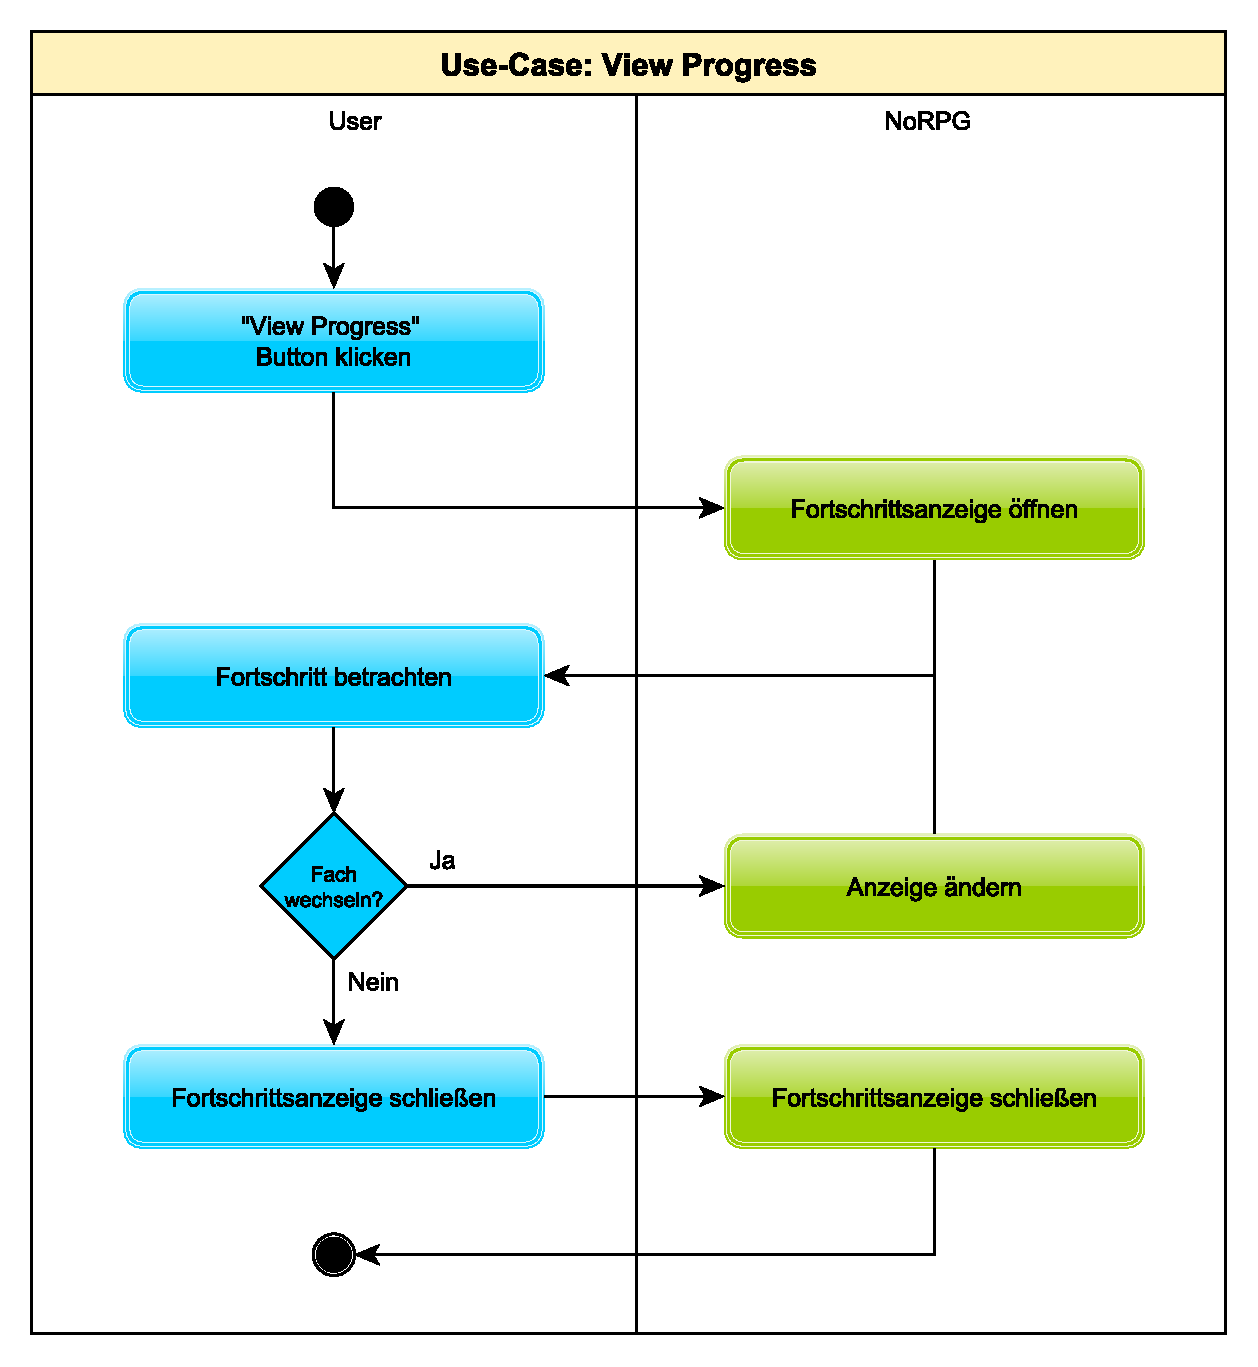
\includegraphics[width=10cm]{pics/ViewProgress.pdf}
				\caption{Activity Diagramm: View Progress}
			\end{figure}
	
			Dieser Use Case hat die gleichen Vorbedingungen wie der vorherige. Der Spieler muss sich im Spiel befinden, darf in keiner aktiven \ac{NPC} Interaktion sein und das Menü ist vorher offen.
	
		\subsubsection{View achievements}
			Dieser use Case beschreibt den Anwendungsfalls, dass der Spieler seine Sammelgegenstände betrachten will. Neben den Standards kann der Anwender im Spiel Gegenstände finden, die ihn in der in Kapitel 2 beschriebenen Story weiterbringen. Diese Collectables sind auf den einzelnen Spielwelten verteilt und können dann, nachdem diese gefunden sind in der Ansicht zusammen mit den anderen betrachtet werden.
			
			Im Prinzip ist dieses Activity Diagramm der gleiche wie der von Use Case "View progress". Der Spieler will seinen Fortschritt betrachten. Dieses mal allerdings seinen Fortschritt in NoRPG. Hier kann der Spieler zwischen den Welten wechseln anstatt zwischen den Fächern und es wird keine Baumstruktur präsentiert.
			
			\begin{figure}[htbp]
				\centering 
				\label{umlAchievements}
				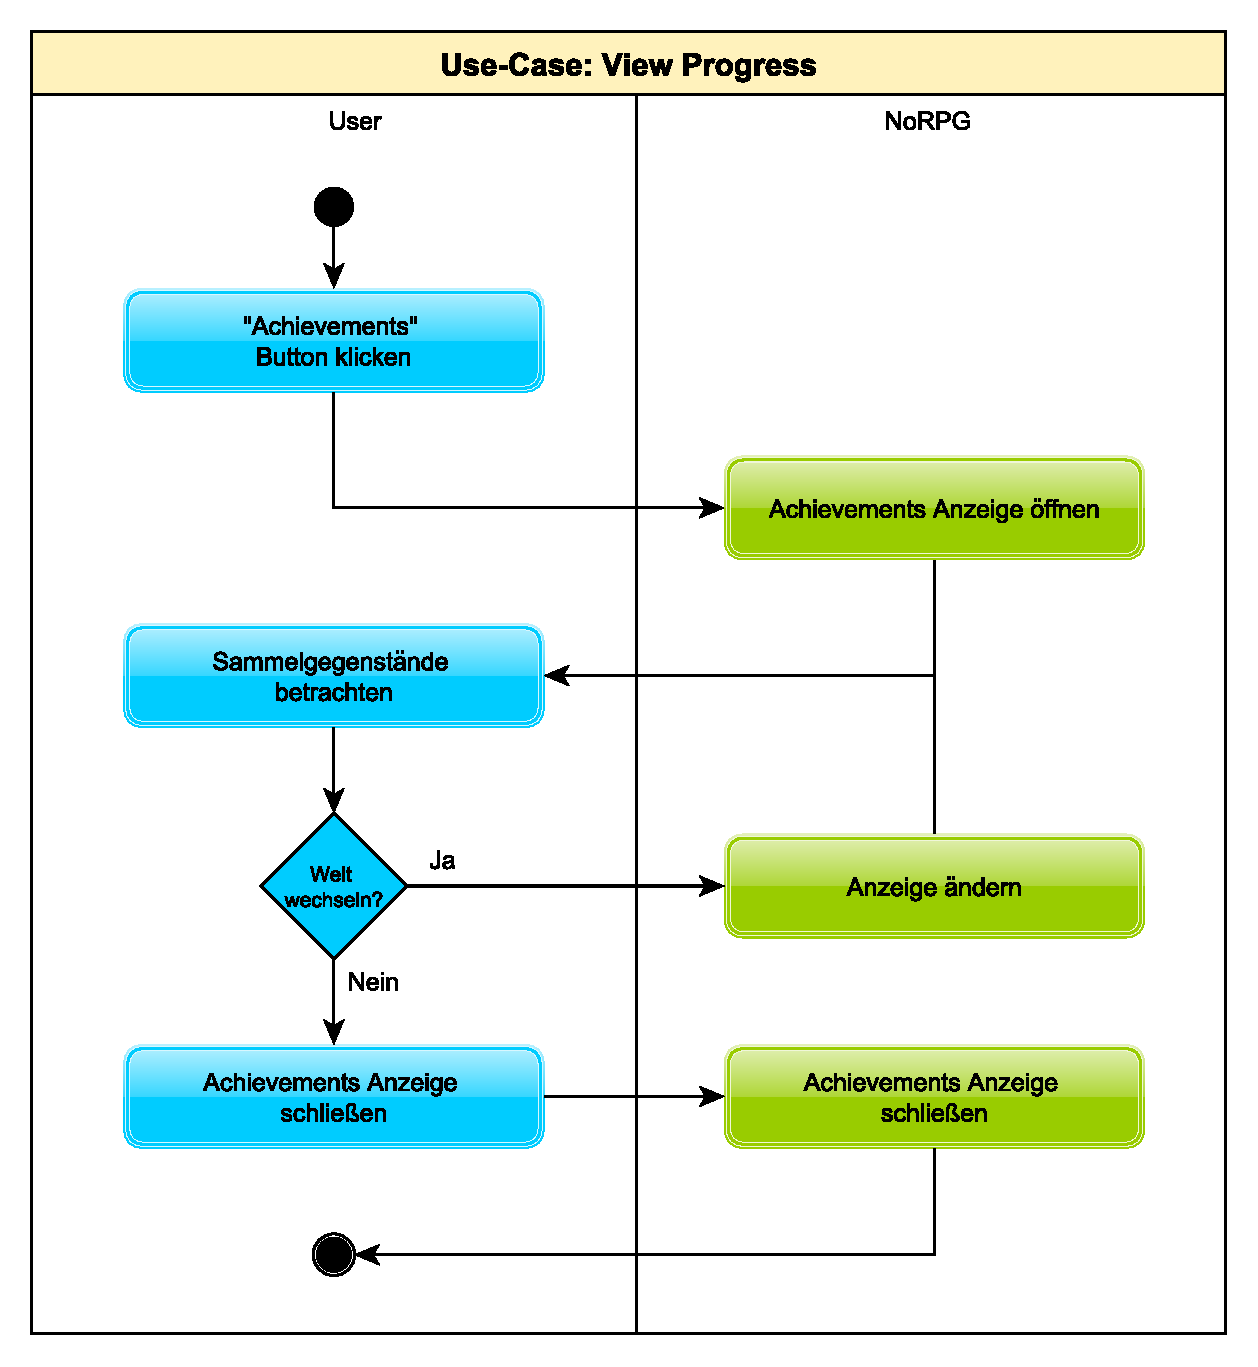
\includegraphics[width=10cm]{pics/Achievements.pdf}
				\caption{Activity Diagramm: Achievements}
			\end{figure}
			
			Dieser Use Case hat die gleichen Vorbedingungen wie der vorherige. Der Spieler muss sich im Spiel befinden, darf in keiner aktiven \ac{NPC} Interaktion sein und das Menü ist vorher offen.
		
		\subsubsection{Change settings}
			Dieser Use Case beschreibt den Anwendungsfall, dass der Benutzer Einstellungen ändern möchte. In dem Rahmen dieser Studienarbeit wird es zwei Einstellungsmöglichkeiten geben. Der Spieler kann die Qualität des Spieles verändern. Ist die Option "High Quality" an, wird alles in höchster Qualität wiedergegeben. Ist jedoch diese Option aus, werden Hintergrundanimationen, die ressourcenaufwändig sind, nicht wiedergegeben. Diese Option ermöglicht es Smartphones mit schlechterer Hardwareausführung das Spiel ohne Probleme spielen zu können, bietet jedoch für neuere Smartphones die Möglichkeit NoRPG in vollen zu genießen.
			
			Die zweite Einstellungsmöglichkeit ist, dass der Spieler die Audioausgaben des Spieles verändern kann. Zu einem Spielerlebnis gehört die Musik und Soundeffekte. Diese kann der Spieler je nach Wunsch ein- oder ausschalten.

			Die Vorbedingung zur Änderung der Spieleinstellungen sind, dass der Anwender sich im Spiel und sich in keiner aktiven \ac{NPC} Interaktion befindet. Bei erfolgreicher Änderung sollten diese Einstellungen für diesen Account gespeichert werden, damit diese bei jedem Login, auch auf verschiedene Geräte, übernommen werden. Im Fehlerfall werden die Default-Optionen angewendet. 
	
		\subsubsection{Save local}
			Dieser Use Case beschreibt den Anwendungsfall, dass der Benutzer seinen aktuellen Fortschritt manuell speichern möchte. NoRPG speichert bei bestimmten Ereignissen automatisch. Beispielsweise wenn der Spieler in eine andere Welt reist oder eine Truhe findet. Allerdings kann der Spieler seinen aktuellen Stand speichern. Es werden neben Fortschritt, Erfolge oder Charaktereigenschaften noch die Spieleinstellungen und sogar der aktuelle Standort des Spielers gespeichert. Der Spieler kann diese Funktion direkt im Menü durchführen.
		
			Wenn das Speichern erfolgreich war, wird der Spieler durch eine kurze Nachricht informiert. Wenn keine Information erscheint kann davon ausgegangen werden, dass der Vorgang fehlgeschlagen ist. Im Fehlerfall muss die Aktion erneut durchgeführt werden.
		
		\subsubsection{Synchronize}
			Dieser Use Case beschreibt den Anwendungsfall, dass der Benutzer seinen lokalen Speicherstand mit dem Server manuell synchronisieren möchte. NoRPG synchronisiert automatisch, wenn eine aktive Internetverbindung vorhanden ist beim Einloggen und vor dem Ausloggen. Die Synchronisation wird nicht so oft wie das Speichern ausgeführt, da der Vorgang länger dauert. Ebenfalls wird die Synchronisation nicht so häufig benötigt, da der Server als eine Art Back-Up verwendet wird. Also für den Fall, dass der Spieler sich mit einem anderen Gerät anmelden möchte. Der Spieler kann diese Funktion direkt im Menü durchführen.
	
			Wenn das Synchronisieren erfolgreich war, wird der Spieler durch eine kurze Nachricht informiert. Wenn keine Information erscheint kann davon ausgegangen werden, dass der Vorgang fehlgeschlagen ist. Eine häufige Ursache für den Fehlschlag kann die fehlende Internetverbindung sein.
		
		\subsubsection{Control character}
			Dieser Use Case beschreibt den Anwendungsfall, dass der Spieler seinen Charakter in NoRPG durch die Spielwelt kontrollieren möchte. Dafür verwendet der Spieler das Steuerkreuz, welches sich in der linken unteren Ecke des \ac{HUD} befindet (vgl. Abbildung \ref{mockupHUD}).
			
			Das Activity Diagramm dieses Use Cases in Abbildung \ref{umlControl} ist im Vergleich zu den bisherigen Diagrammen besonders, denn es existiert keinen Endpunkt. 
			
			\begin{figure}[htbp]
				\centering 
				\label{umlControl}
				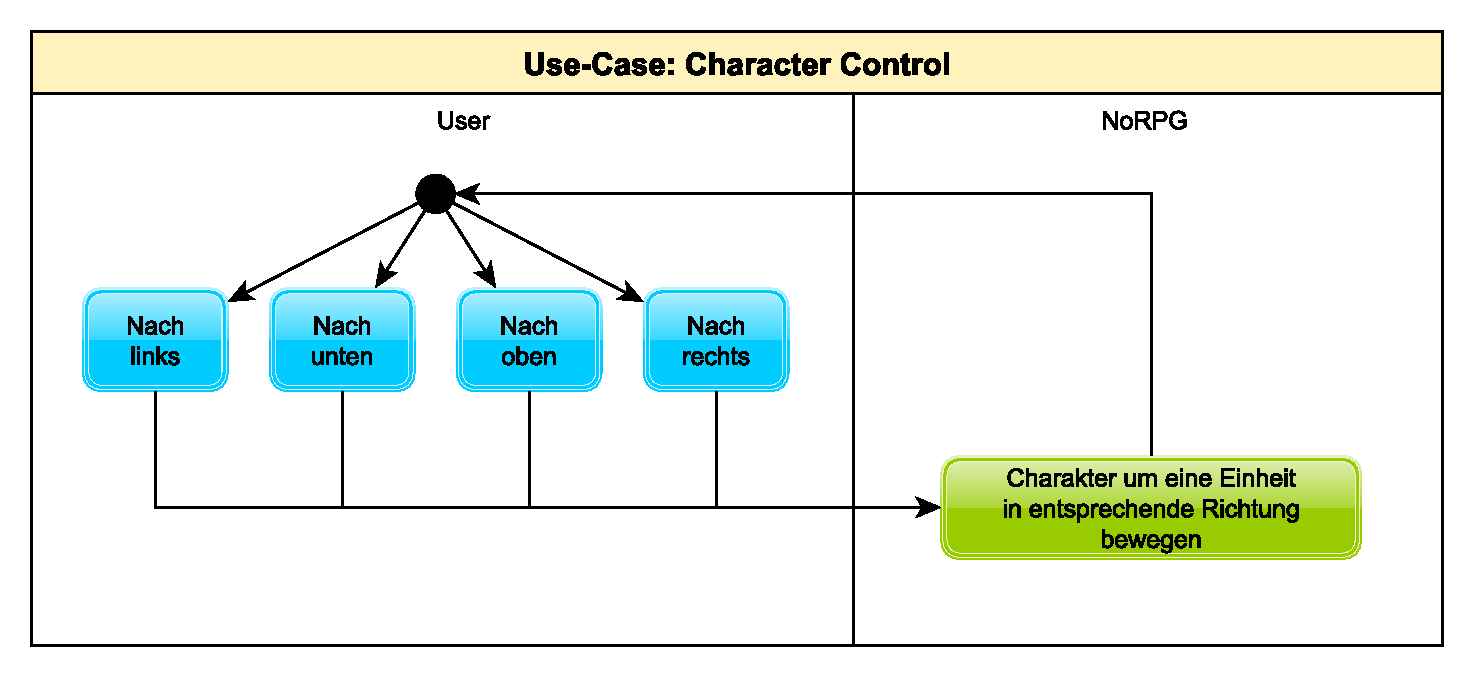
\includegraphics[width=13cm]{pics/CharacterControl.pdf}
				\caption{Activity Diagramm: Character Control}
			\end{figure}
		
			Wenn der Spieler das Steuerkreuz nach oben bewegt, wird der Charakter des Spielers um eine Einheit nach vorne bewegt. Nach dem Abschluss dieser Aktion kann der Spieler den Charakter direkt weiter bewegen. Wenn der Touchscreen in eine Richtung gehalten wird, dann wird dieser Ablauf ganze Zeit durchgeführt, bis die Touchscreen losgelassen wird.
			
			Die Vorbedingung für diesen Use Case ist, dass der Spieler sich im Spiel befindet und das Menü geschlossen ist.
	
		\subsubsection{Interact with elements}
			Dieser Use Case beschreibt den Anwendungsfall, dass der Benutzer mit einen Element im Spiel interagieren möchte. Dafür hat der Spieler 2 Tasten auf dem \ac{HUD} (vgl. Abbildung \ref{mockupHUD}), die dem Spieler die Möglichkeit gibt die Interaktion zu starten oder zu beenden.
			
			In NoRPG wird es verschiedene Elemente geben, mit denen der Spieler interagieren kann.
			
			\begin{itemize}
				\item {\textbf{\acp{NPC}:} Der Spieler kann sich mit unterschiedlichsten \acp{NPC} unterhalten, die überall in allen Spielen vorkommen. Die \acp{NPC} helfen dem Spieler, indem diese Tipps und Hinweise in den Unterhaltungen nennen.}
				\item {\textbf{Truhen:} Der Spieler kann mit Truhen interagieren. Die Truhen sind in den einzelnen Welten verteilt und enthalten die Sammelgegenstände. Durch die Interaktion öffnet sich die Truhe und der Sammelgegenstand erscheint. Nachdem die Truhe geöffnet wurde bleibt die Truhe offen und es kann nicht weiter mit ihr interagiert werden. Es handelt sich um eine einmalige Aktion.}
				\item {\textbf{Spielehändler:} Spielehändler tauchen überall auf. Diese bieten die verschiedenen Lernspiele für Standards an. Die Spielehändler können menschliche Händler oder andere Formen annehmen um die verschiedene Welten zu repräsentieren. Durch die Interaktion startet der Spieler eine Unterhaltung in dem der Spieler Informationen über den Standard erhält und das Spiel freischaltet.}
				\item {Die Interaktion mit der Umwelt (Bäume, Tiere, Gebäude) starten zunächst keine Aktion.}
			\end{itemize}
			
			Eine Interaktion kann nur dem "A" Button gestartet werden. Wenn ein Element zur Interaktion vorhanden ist startet erst die Interaktion. Anschließend kann der Spieler mit dem "A" oder "B" Button reagieren. Der "B" Button ist zum Abbrechen der Interaktion und beendet diesen Prozess bzw. überspringt ihn. Zum Beispiel in der Interaktion mit dem Händler sorgt der "B" Button dafür, dass die Unterhaltung übersprungen wird und direkt die Spiele angezeigt werden. Mit dem "A" Button wird die Interaktion fortgeführt bis keine Aktion mehr vorhanden ist, also in unserem Händlerbeispiel keine Unterhaltung mehr gibt.
			
			\begin{figure}[htbp]
				\centering 
				\label{umlInteraction}
				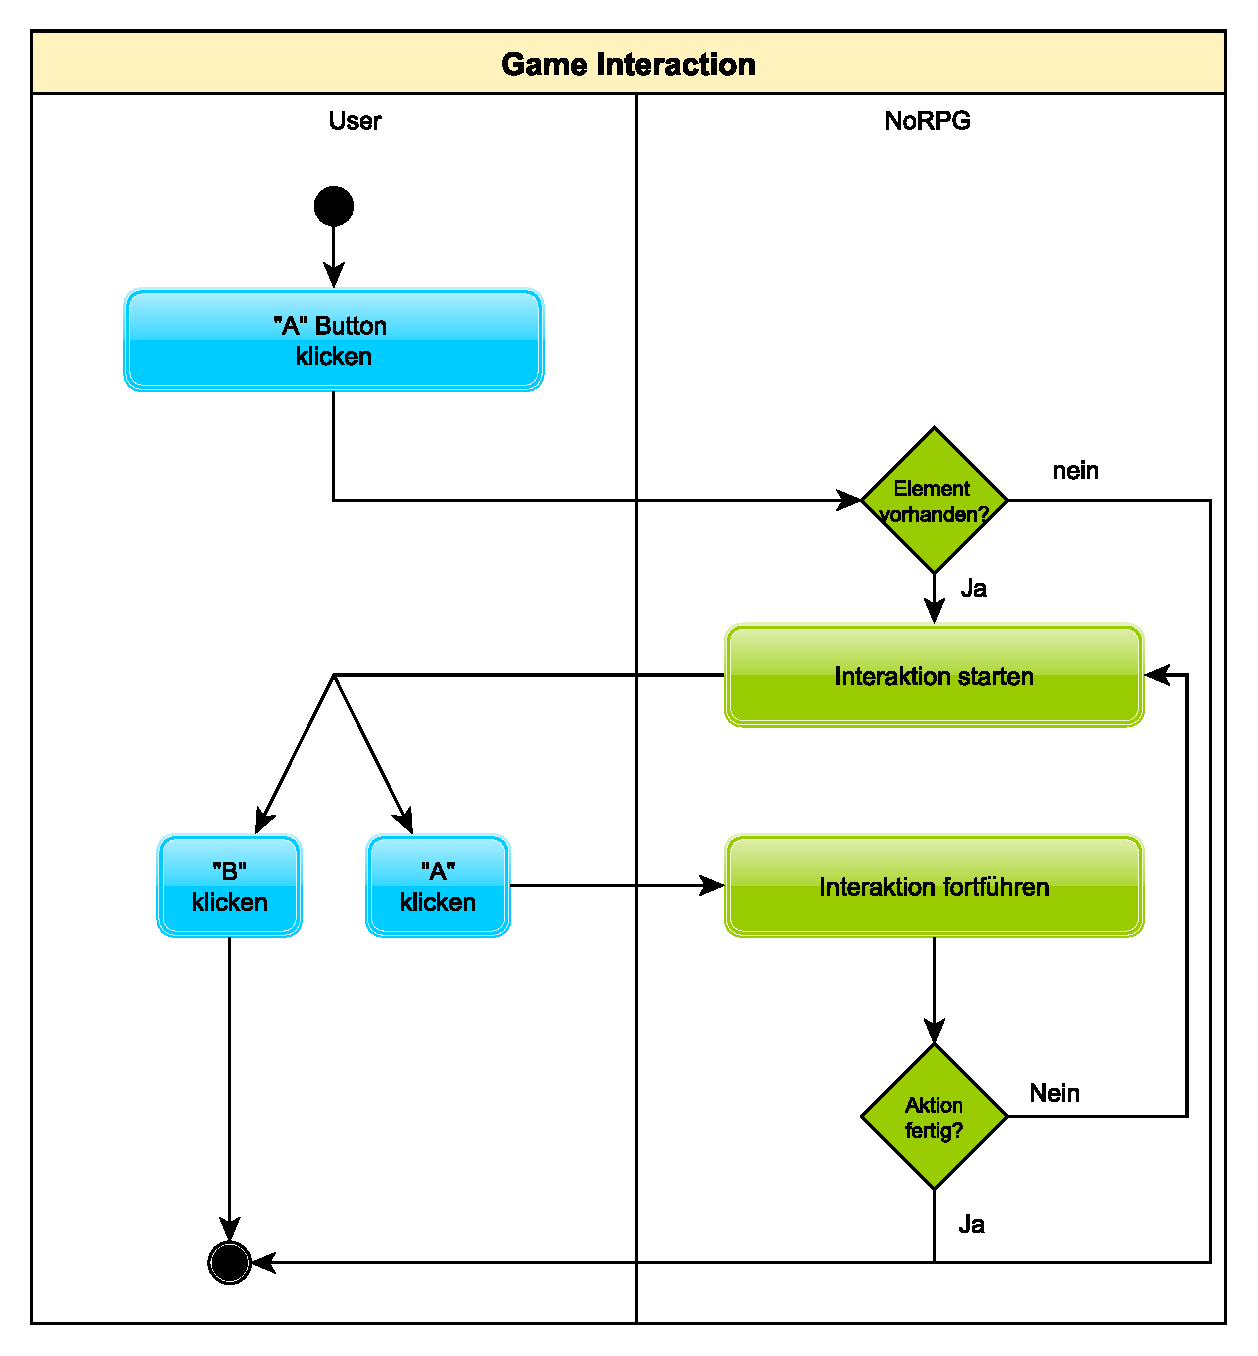
\includegraphics[width=10cm]{pics/GameInteraction.pdf}
				\caption{Activity Diagramm: Game Interaction}
			\end{figure}
			
			Die Vorbedingungen für diesen Use Case sind, dass der Spieler sich im Spiel befindet und das Menü sowie die Karte geschlossen sind. Je nach Element wird ein anderes Ergebnis erwartet. Beispielsweise wird bei einer Interaktion mit der Truhe das Ergebnis erwartet, dass die Truhe offen bleibt, der Sammelgegenstand in die Liste übernommen wurde und der Spielstand automatisch lokal gespeichert wird.
	
	\subsection{Performanz Anforderungen}
		Dieser Abschnitt des \ac{SRS} legt sowohl die statischen als auch die dynamischen numerischen Anforderungen an die Software. 
	
		Ein sehr wichtige Anforderung betrifft die Antwortzeit des Systems. Diese Anforderung ist besonders wichtig, da der Nutzer die direkten Auswirkungen in der App mitbekommt. Eine Antwortzeit von 0,1 Sekunden gibt dem Benutzer das Gefühl, dass das System sofort reagiert. Bei einer Sekunden denkt der Benutzer immer noch, dass die Aktion ununterbrochen durchgeführt wird, jedoch bemerkt der Benutzer ein Verzögern. Im Worst-Case liegt die Grenze für die Aufmerksamkeit des Benutzers bei zehn Sekunden\footnote{vgl. Andrew Lee \cite{performance1}}.
		
		Für die Performanz Anforderungen wird zwischen der App und dem Server unterschieden. 95\% der Transaktionen in der App sollten in weniger als einer Sekunde verarbeitet werden. Aufwändigere Prozesse wie die Synchronisation oder das wechseln der Spielwelten dürfen minimal länger brauchen. Für den Server gilt, dass 80\% der Transaktionen in weniger als einer Sekunde verarbeitet werden. Es sind nur 80\% notwendig, da der Server nur für die Synchronisation und Speicherung verwendet wird. Der prozentuale Anteil der Synchronisation auf dem Server ist wesentlich größer als die in der App. 
		
		Der Workload ist die Anzahl an Verarbeitungen, die das System in einer gegeben Zeit durchführen kann. Die App selbst hat keine hohe Arbeitsbelastung, da diese nur einen Benutzer gleichzeitig zulässt und von der Hardware des Spielers abhängt. Vielmehr gilt es zu betrachten, mit wie viel Belastung der Server umgehen kann. Der Anzahl an Spielern ist mehr oder weniger keine Grenze gesetzt, da für jeden einzelnen Spieler zunächst eine Zeile in der Datenbank hinterlegt wird. Die Anzahl an gleichzeitigen Benutzern, die mit dem Server kommunizieren wollen, ist allerdings begrenzt. Da der Server auch sein Hardwarebegrenzungen hat kann es nur eine bestimmte Anzahl an gleichen Synchronisationsanfragen entgegennehmen. Wenn diese Anzahl übersteigt wird arbeitet der Server nach dem First In First Out (FIFO) Prinzip. Die Clients, die als erste eine Synchronisationsanfrage senden, werden auch als erstes bearbeitet. Als eine Art der Erweiterung spezifiziert die Lastskalierbarkeit die Menge an Daten, die innerhalb bestimmter Zeitperioden sowohl bei normaler als auch bei maximaler Belastung verarbeitet werden sollen.

	\subsection{Datenbank Anforderungen}
		Die beiden eingesetzten Datenbanken unterscheiden sich von ihren Anforderungen.
		
		Bei der Datenbank in der App handelt es sich um eine embedded, zu deutsch eingebettete, Datenbank. Sie wird zusammen mit der App ausgeliefert. Die Datenbank enthält zunächst die Spieldaten. Das ist eine Liste der Standards mit den dazugehörigen Spielen. Neben diesen Daten werden lokal noch die Daten des Spielers gespeichert. Die Spielerdaten beinhalten gespeicherte Einstellungen, die Charaktereigenschaften und den Fortschritt. Dadurch wird das Spielen ohne eine aktive Internetverbindung ermöglicht.
		
		Die embedded Datenbank wird oft verändert, da bei jedem Fortschritt automatisch gespeichert wird. Zudem werden die Daten der Datenbank beim Einloggen und vor dem Ausloggen immer mit dem Server synchronisiert. Die Daten werden beim Ausloggen gelöscht, damit sich verschiedene Spieler auf einem Smartphone anmelden können und die Datensicherheit gewährleistet wird.
		
		Die Integrität der Datenbank muss immer gewährleistet werden, damit die Benutzer den eigenen Fortschritt nicht fälschen können. Dies kann mit Prüfsummen und Versionierung gewährleistet werden.
		
		Die Datenbank auf dem Server enthält alle Spielerdaten und Spieldaten. Bei den Spieldaten handelt es sich um die gleichen Daten, die auf den lokalen Datenbanken gespeichert sind.  Allerdings sind auf dem Server alle Spielerdaten gespeichert, damit die Benutzer von unterschiedlichen Geräten spielen können. 
		
		Diese Datenbank wird nicht oft verändert bzw. aktualisiert, da die Datenbank nur bei der Synchronisation verändert wird oder wenn neue Standards oder Spiele eingefügt werden. Das hat den Vorteil das nicht sehr viele Anfragen an den Server gestellt werden, wodurch der Workload gering gehalten wird. Zugegriffen kann der Spieler nur über die App. Administratoren haben die Möglichkeit den Server über eine Virtual Machine zu erreichen und Änderungen durchzuführen. 
		
		Auch hier muss die Integrität der Datenbank immer gewährleistet werden.
	
	\subsection{Entwurfsbeschränkungen}
		Bei der Entwicklung der App gilt es zu beachten, dass die Hardware-Anforderungen nicht zu hoch sind. Als Maßstab für die Hardware wird das Smartphone Samsung Galaxy S4 genommen. Grund dafür ist das Preis-Leistungsverhältnis des S4 und die Tatsache, dass Samsung eine sehr verbreitete Marke ist.
		
		Das Samsung Galaxy S4 kostet auf Amazon (Stand 27.01.2017) ungefähr 225 Euro. Das S4 hat vorinstalliert Android 4.2 Jelly Bean und die Samsung Touchwiz 4.0 Oberfläche. Ein Update auf Android 5.0 Lollipop ist allerdings möglich. Das S4 hat 2 GByte Arbeitsspeicher und 16 GByte internen Speicher, welcher durch eine Speicherkarte erweitert werden kann. Bei dem Prozessor handelt es sich um einen Qualcomm Snapdragon 600 mit vier Kernen, einer Taktfrequenz von 1,9 GHz und einer 32-bit Architektur\footnote{vgl. Google \cite{s4Google}}. Für eine Internetverbindung bietet Samsungs Galaxy S4 eine drahtlose Schnittstelle, die nach IEEE 802.11a/ac/b/g/n funktioniert.
		
		Der Speicherbedarf darf nicht größer als 200MB sein, geplant sind allerdings 150MB. Beim RAM dürfen nicht mehr als 1GB sein, geplant sind allerdings 500MB.
	
	\subsection{Benutzerfreundlichkeit}
		Das Ziel der Benutzerfreundlichkeit ist eine hohe Ergonomie. Die Software-Ergonomie bezeichnet die Anpassung an die kognitiven und physischen Fähigkeiten bzw. Eigenschaften des Benutzers, also seine Möglichkeiten zur Verarbeitung von komplexen Informationen aber auch die Anpassung softwaregesteuerten Merkmale der Darstellung, wie Farben und Schriftgröße.
		
		Damit die Benutzeroberfläche freundlich für den Benutzer ist, muss sie in das Profil des Benutzers passen. Da NoRPG sich grundsätzlich an Kinder richtet muss die Bedienung und Gestaltung der App kindgerecht sein. Damit eine App als kindgerecht bezeichnet werden kann muss es nach Wendy B. von Intel vier Prinzipien erfüllen \footnote{vgl. Wendy B. \cite{intelKids}}.
		
		\begin{enumerate}
			\item{Freiheit: Die Fähigkeit, sich in der App innerhalb einer kontrollierten Umgebung frei bewegen zu können. Dieses Prinzip verfolgen auch Rollenspiele. Durch die offene Spielwelt kann der Spieler selbst entscheiden wohin er als nächstes hin möchte. Allerdings gilt es bei Kindern diese Umgebung zu kontrollieren, indem bestimmte Bereiche festgelegt werden müssen.}
			\item{Komfort: Die App sollte stimulieren, jedoch darf es nicht übertrieben werden. Dies wird als Balanceakt bezeichnet. Abwechslungsreiche Stimulationen sind definitiv notwendig, beispielsweise durch die Animationen, Farben oder Musik. Dadurch wird die Wahrnehmung und Aufmerksamkeit erhöht. Allerdings ist die Linie zwischen Stimulation und Lärm bzw. zu viel Stimulation sehr dünn und kann leicht überschritten werden.}
			\item{Vertrauen: Kinder, genau wie Erwachsene, müssen sich kompetent fühlen und wollen ihren Aktionen vertrauen.}
			\item{Kontrolle: Kinder wollen das Gefühl, dass sie etwas vollbringen wenn sie in der App interagieren. Es werden Ziele gesetzt und Entscheidungen getroffen.}
		\end{enumerate}
	
		Für die kindgerechte Gestaltung gibt es allerdings noch weitere Kriterien. Es dürfen keine In-App-Käufe angeboten, keine Werbung platziert oder zu Social Media oder ähnlichen Seiten verlinkt werden. Diese Gegenstände haben in einem kindgerechten Spiel nichts zu tun. Für die Installation gilt es zu beachten, das so wenig Berechtigungen wie notwendig verlangt werden\footnote{vgl. klick-tipps.net \cite{appsforkids}}.
		
		Es gilt, desto einfach die App gestaltet ist, desto mehr Kinder verstehen diese. Ein Beispiel dafür ist die Charaktersteuerung. Moderne Spiele haben keine sichtbaren Steuerkreuz, der Spieler muss nur eine Ziehbewegung in die Richtung machen, in der er sich bewegen möchte. In NoRPG allerdings wird ein sichtbares Steuerkreuz gewählt, wie dies schon von vielen Geräten wie vom klassischen Gameboy oder von Playstation verwedent wird. Navigation soll schnell erkennbar und nachvollziehbar sein.
		
		Schließlich gilt es die erwachsenen Nutzer nicht zu vergessen! Gemeint sind Eltern, Erziehungsberechtigte, Lehrer und jeder, der mit der App interagieren kann. Erwachsene spielen genauso eine wichtige Rolle. Egal ob diese die Kinder unterstützen, überwachen oder selbst spielen. Es ist wichtig, dass sich Eltern an die Entwickler melden können, wenn sie etwas nicht kindgerecht halten oder wenn es Probleme gibt\footnote{vgl. Becky White \cite{smashMagazin}}.	

	\subsection{Zuverlässigkeit}
		Alle implementierten Produktfunktionen sollten zur Auslieferung korrekt und zuverlässig funktionieren. Dazu zählt auch, dass die Funktionen in vertretbaren Zeiten terminieren. Beispielsweise sollte die Anmeldung funktionieren, wenn der Spieler registriert ist und die richtigen Benutzerdaten eingegeben hat, oder die Benutzereingaben für die Charaktersteuerung sollen korrekt interpretiert werden.
		
		Eine besondere Wichtigkeit hat die Implementierung der in Kapitel 2 beschriebenen \acp{CCSS}. Diese sind wichtig für die Reihenfolge der spielbaren Lernspiele, damit ein Spieler mit einem Skilllevel der ersten Klasse in Geometrie keine Lernspiele für die fünfte Klasse angezeigt kriegt. Erst dadurch wird gewährleistet und kann sichergestellt werden, dass der Spieler die Lerninhalte korrekt vermittelt kriegt.
	
	\subsection{Verfügbarkeit}
		Da bei jeder App eine lokale Datenbank vorhanden ist, muss der Server nicht die ganze Zeit verfügbar sein. Das gilt jedoch nur für die Benutzer, die NoRPG schon heruntergeladen und sich angemeldet haben. Wenn diese Bedingungen erfüllt sind, wird der ganze Fortschritt lokal gespeichert und kann mit dem Server manuell oder automatisch synchronisiert werden. Für den Fall, dass der Benutzer sich von einem anderen Gerät anmelden möchte, muss der Server verfügbar sein.
		
		Daher werden nur die Verfügbarkeit des Logins bzw. Registrierung und der Synchronisation bewertet. Der Login muss eine Verfügbarkeit von 99\% haben, wohingegen bei der Synchronisation eine Verfügbarkeit von 90\% ausreicht.
		
	\subsection{Sicherheit}
		Bei Sicherheit wird zwischen zwei unterschiedlichen Typen unterschieden: Security und Safety. Security ist der Schutz vor absichtlichen Bedrohungen, wenn ein Angreifer absichtlich das Systems angreift. Im Gegensatz dazu ist Safety der Schutz vor unbeabsichtigten Bedrohungen, wenn der Benutzer durch Zufall die Sicherheitsmechanismen umgeht indem er etwas nicht beabsichtigtes ausführt.
		
		Die Kommunikation mit dem Server und mit der lokalen eingebetteten Datenbank müssen verschlüsselt werden, damit die Credentials bei den Anmeldung oder bei der Registrierung nicht mitgelesen werden können. Des Weiteren müssen die Daten auf der lokalen Datenbank validiert werden, bevor der Server synchronisiert wird, denn es wird unter anderem auch der Spielfortschritt der Benutzer synchronisiert. Die Veränderung des Spielfortschritts wird als Schummeln bzw. Cheaten behandelt.
		
		Die Anmeldung bzw. Registrierung ist notwendig, um NoRPG spielen zu können. Deswegen müssen die Accounts der Benutzer verschlüsselt gespeichert werden und die Passwörter dürfen bei der Anmeldung nur mittels One-Way-Functions vergleichen werden. Nicht registrierte bzw. unautorisierte Benutzer erlangen keinen Zugriff auf das System.
		
		Die gespeicherte Daten dürfen an andere Tools nur anonymisiert weitergegeben werden, für beispielsweise Analysezwecke. Diese Kommunikation mit anderen System oder Applikationen darf nur verschlüsselt geschehen.
		
	\subsection{Wartbarkeit}
		Der Code von NoRPG sollte so geschrieben werden, dass der Code die Umsetzung neuer Funktionen begünstigt. Deshalb sollte die Komplexität des Quellcodes so gering wie möglich gehalten werden, indem entsprechende Methoden wie das Model-View-Controller (MVC) Pattern umgesetzt werden. Des Weiteren sollte das System von NoRPG Schnittstellen jeglicher Art anbieten, um das System durch weitere Komponenten wie ein Web-Tool für Administratoren zu erweitern.
		
		Neben der Erweiterbarkeit sollte NoRPG für Fehlerfälle eine Testumgebung anbieten, um das Testen der Anwendung auf unterschiedliche Funktionen zu ermöglichen und gegebenenfalls Fehler wiederholen und simulieren zu können.
		
	\subsection{Portabilität}
		Die App NoRPG ist zunächst nur für Android geplant. Andere Betriebssysteme, wie Windows Phone von Microsoft oder iOS von Apple, sind vorerst nicht vorgesehen. 
		
		Bei der vorhanden Breite an Varianten von Android-Smartphones ist sehr wichtig, dass die Portabilität innerhalb von Android Smartphones gewährleistet wird. Neben bekannten Smartphoneherstellern wie Samsung, LG oder HTC gibt es zahlreiche weitere Hersteller die auf das Android Betriebssystem setzen. Jeder Hersteller hat dabei eine große Palette an Smartphone-Modellen, wie bei Samsung die Samsung Galaxy S-Reihe, welches aktuell in der siebten Genration erhältlich ist\footnote{vgl. Philippe Fischer, Michael Huch \cite{computerBildSamsung}}, oder die Samsung Galaxy Note-Reihe. Die App NoRPG muss auf allen Android-Smartphones funktionieren, solange diese die Mindestanforderungen an Software und Hardware erfüllen. Dabei muss sich die App beispielsweise an die Auflösung des Smartphones anpassen.
		
		Die Portabilität beschreibt nicht nur die technische Sicht sondern auch in welchen Ländern und in welchen Sprachen NoRPG verfügbar sein wird. Der Release findet in allen Ländern statt, in denen der Google Play Store verfügbar ist. Zunächst wird NoRPG nur in Englisch verfügbar sein.